\section{Qualitative Fehleranalyse}
\label{sec:fehleranalyse}

\subsection{Qualitativer Eindruck}

Abbildung~\ref{fig:bev-vergleich} zeigt denselben Frame einmal aus der Einzelsensoransicht \texttt{os1} und einmal aus der fusionierten Ansicht, jeweils in der Vogelperspektive mit Ground-Truth-Boxen und den Vorhersagen des zugehörigen Foldmodells.

\begin{figure}[H]
\centering
\begin{subfigure}{\textwidth}
\centering
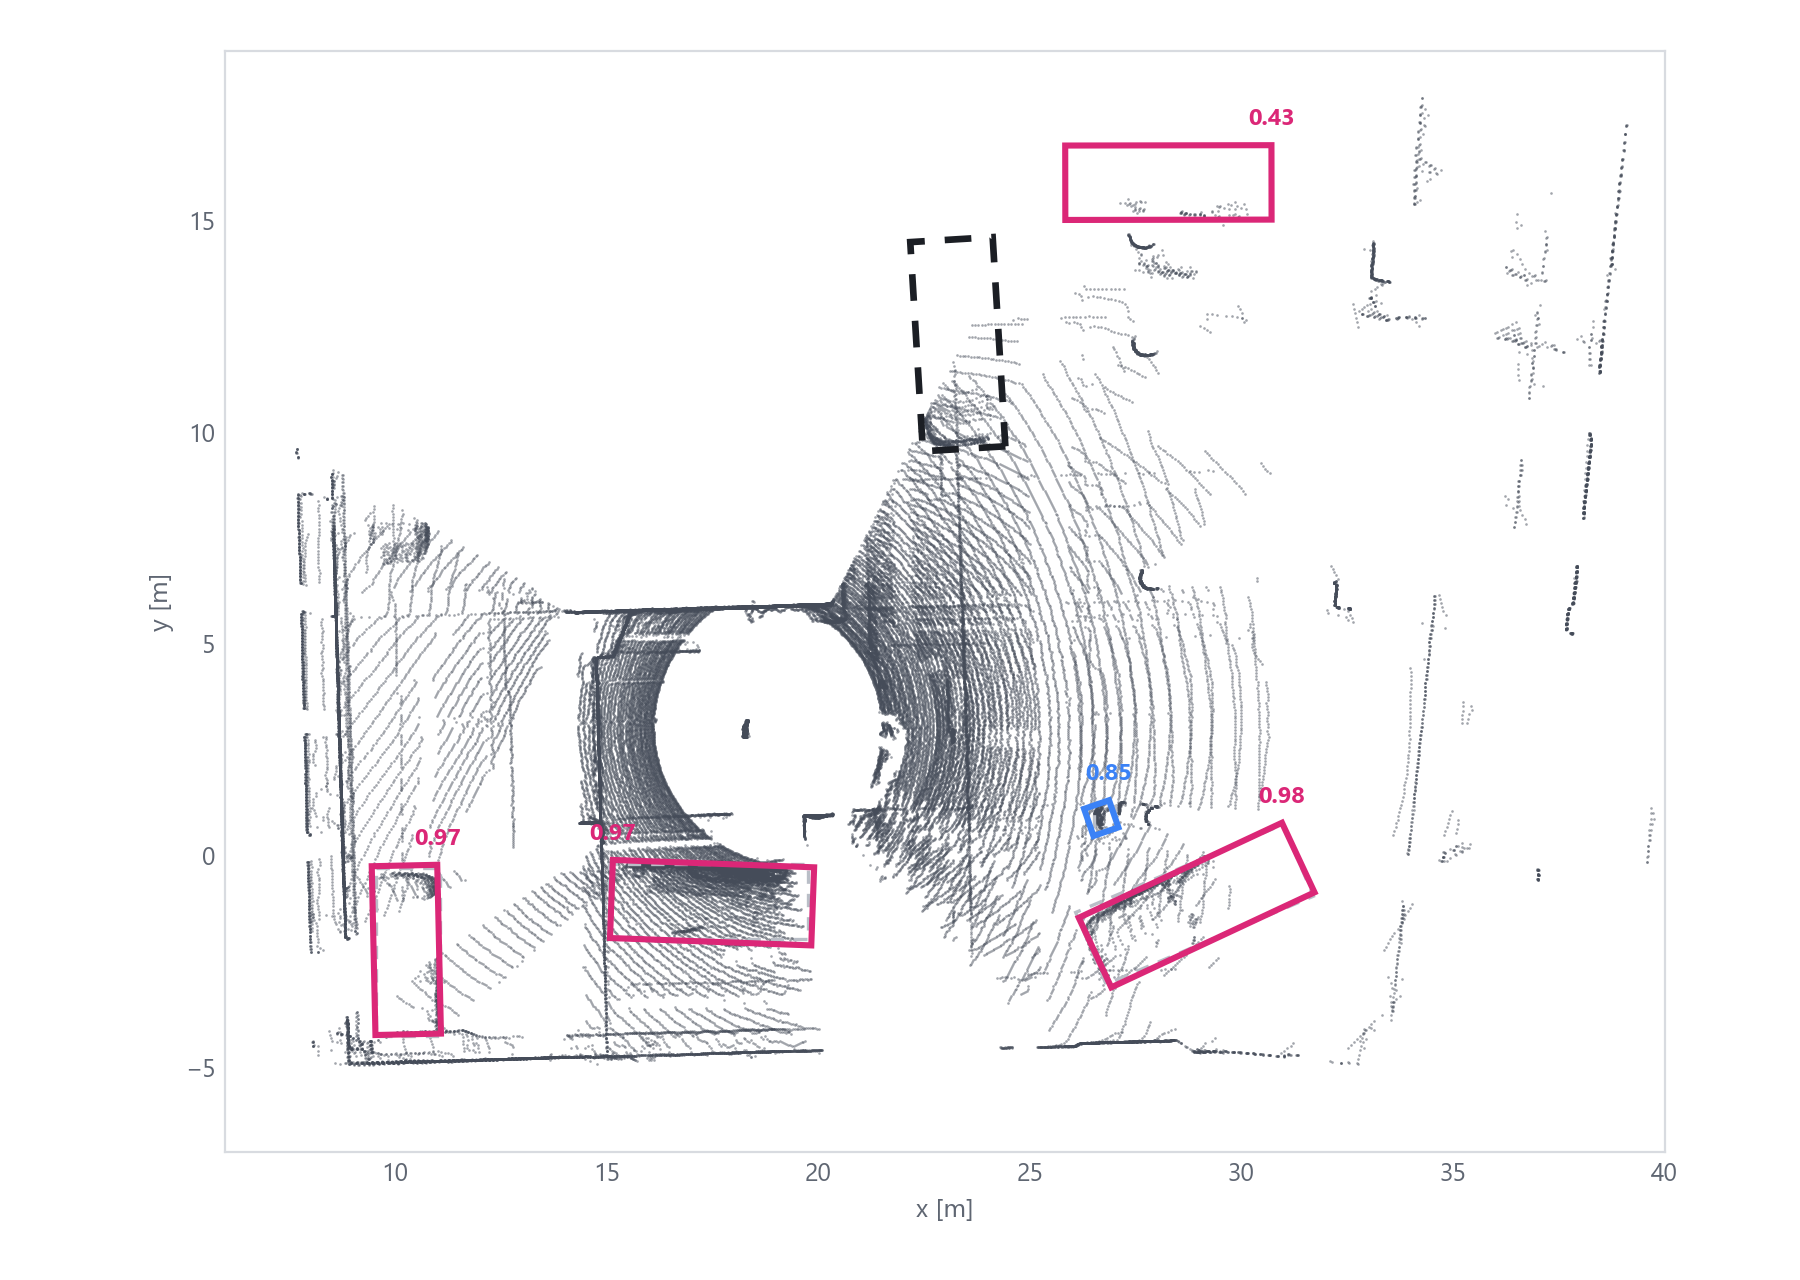
\includegraphics[width=0.62\textwidth]{images/bev-os1.png}
\caption{Einzelsensoransicht \texttt{os1}}
\label{fig:bev-einzel}
\end{subfigure}

\vspace{0.2cm}

\begin{subfigure}{\textwidth}
\centering
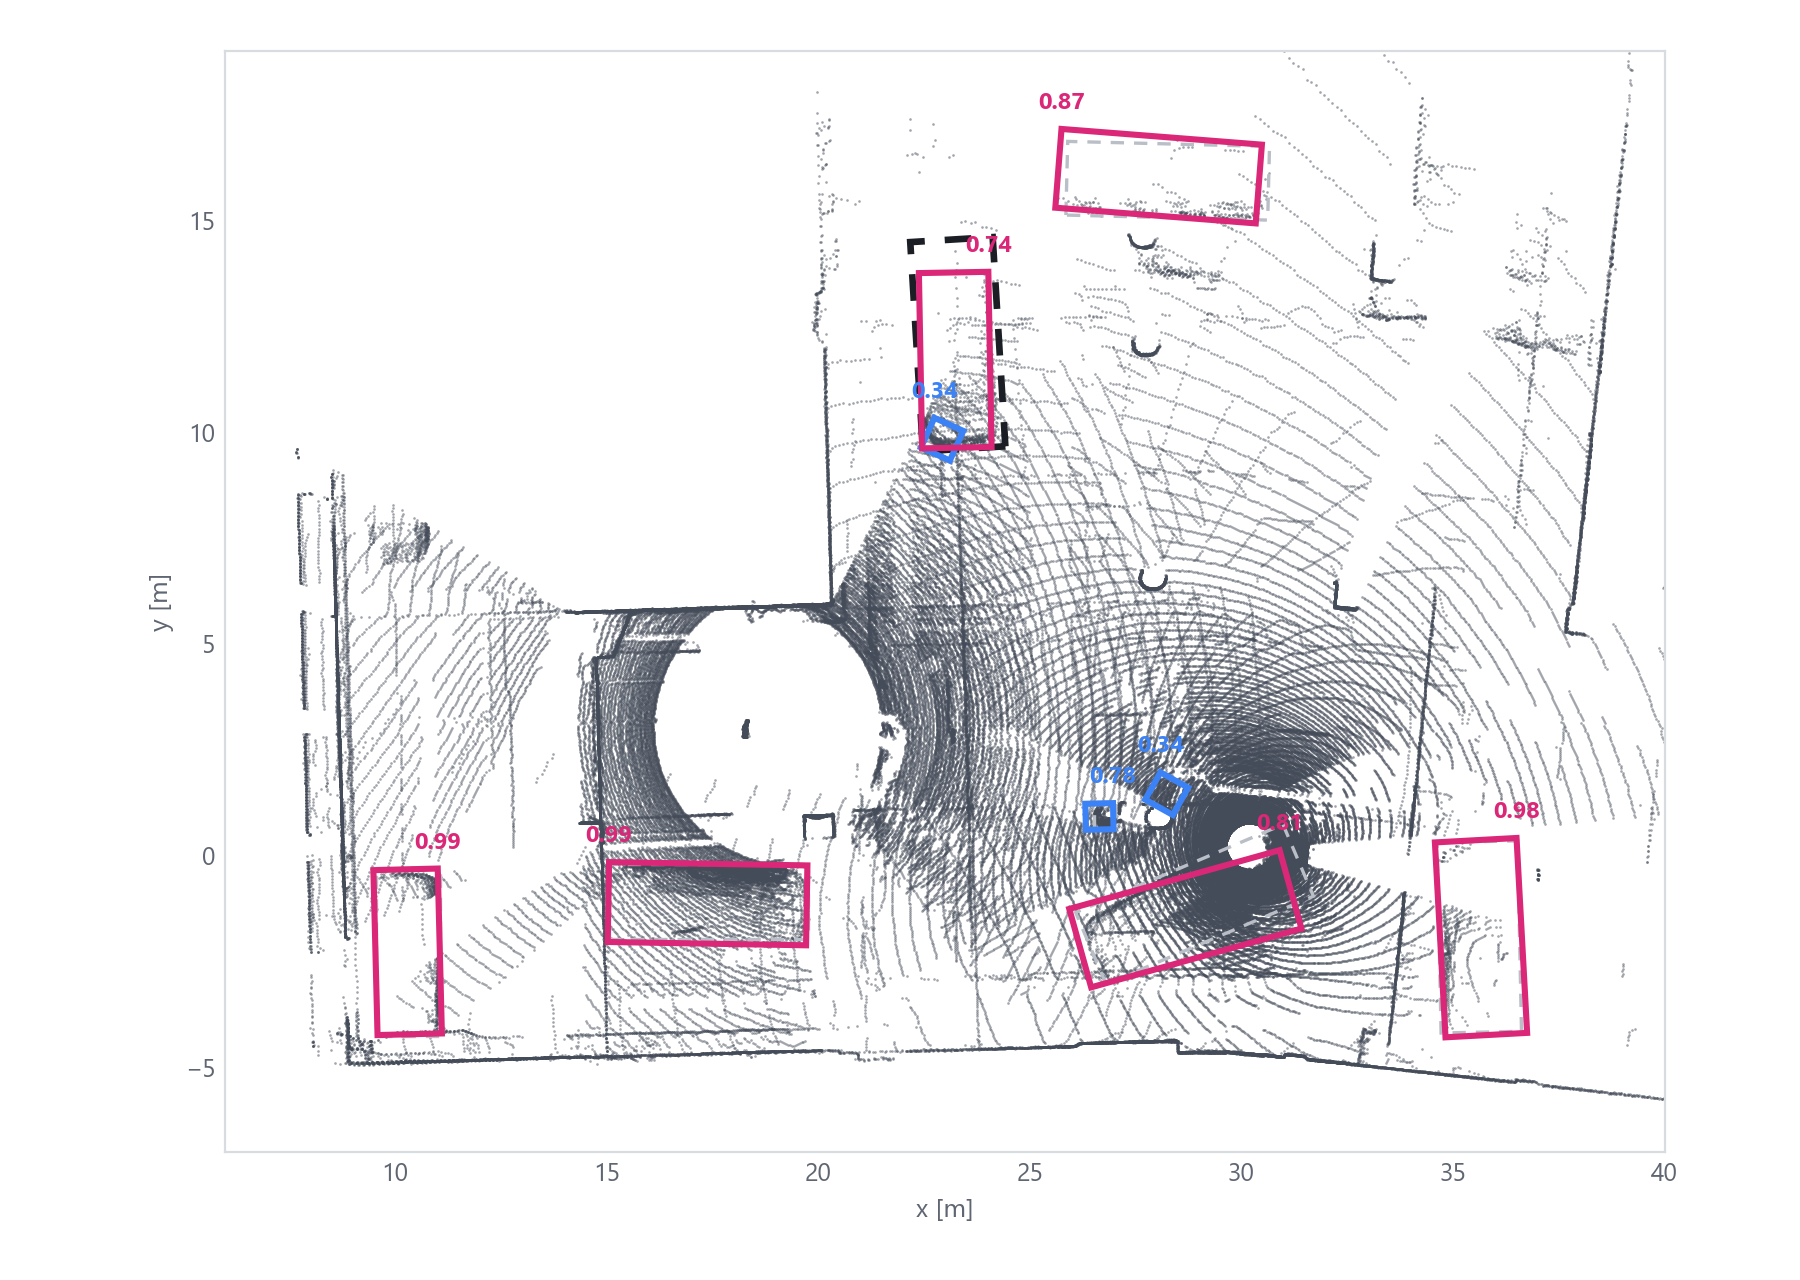
\includegraphics[width=0.62\textwidth]{images/bev-merged.png}
\caption{Fusionierte Ansicht \texttt{merged}}
\label{fig:bev-fusion}
\end{subfigure}
\caption{Derselbe Frame in Vogelperspektive. Gestrichelt: Ground Truth; durchgezogen mit Konfidenzwert: Vorhersagen. In~\subref{fig:bev-einzel} bleibt die gestrichelte Ground-Truth-Box des Autos im oberen Bildbereich ohne zugeordnete Vorhersage, weil das Fahrzeug aus der Perspektive von \texttt{os1} nur wenige Punkte erhält. In~\subref{fig:bev-fusion} ergänzen die Punkte von \texttt{os0} die verdeckte Fahrzeugseite, sodass dort eine Vorhersage entsteht.}
\label{fig:bev-vergleich}
\end{figure}

Das Bild illustriert den Mechanismus hinter dem Fusionsvorteil: Die zusätzliche Perspektive füllt Verdeckungen auf und erhöht die Punktdichte an Objektseiten, die aus einer einzelnen Richtung abgeschattet sind. Der gezeigte Einzelfall passt zum quantitativen Befund, denn \texttt{os1} erreicht beim Auto mit einem AP\textsubscript{30} von 0{,}832 den niedrigsten Wert der drei Ansichten (Tabelle~\ref{tab:moving-objects-ap}).

Zugleich zeigt die Abbildung die Grenze des Effekts, denn die in der fusionierten Ansicht entstehende Vorhersage besitzt nur eine geringe Konfidenz und würde eine übliche Betriebsschwelle nicht überschreiten. Einzelne Frames sind als Beleg ohnehin nicht ausreichend; die quantitative Grundlage bleibt die Cross-Validation.

\subsection{Definition der Geisterboxen}
\label{sec:geisterboxen}

Für die generalisierte OOF-Analyse wird eine Geisterbox als Vorhersage mit Score mindestens 0{,}3 definiert, die sich keiner noch unbenutzten GT-Box derselben Klasse bei 3D-IoU mindestens 0{,}3 zuordnen lässt. Diese Definition umfasst nicht nur leere Halluzinationen, sondern auch Duplikate, falsch klassifizierte reale Strukturen und schlecht lokalisierte Boxen.

Auf den 2.122 gemeinsamen Testframes ergeben sich die in Tabelle~\ref{tab:ghost-boxes} aufgeführten Geisterbox-Zahlen:

\begin{table}[H]
\centering
\begin{tabular}{ccccc}
\toprule
\textbf{Ansicht} & \textbf{Person} & \textbf{Fahrrad} & \textbf{Auto} & \textbf{Gesamt} \\
\midrule
merged & 510 & 315 & 159 & 984 \\
os0    & 948 & 157 & 415 & 1.520 \\
os1    & 329 & 372 & 248 & 949 \\
\bottomrule
\end{tabular}
\caption{Anzahl Geisterboxen (Score \(\geq\) 0{,}3, IoU \(<\) 0{,}3) auf den 2.122 gemeinsamen OOF-Testframes.}
\label{tab:ghost-boxes}
\end{table}

Abbildung~\ref{fig:geisterboxen-rate} normiert dieselben Zahlen auf 100 Frames und macht die Klassenzusammensetzung sichtbar.

\begin{figure}[H]
\centering
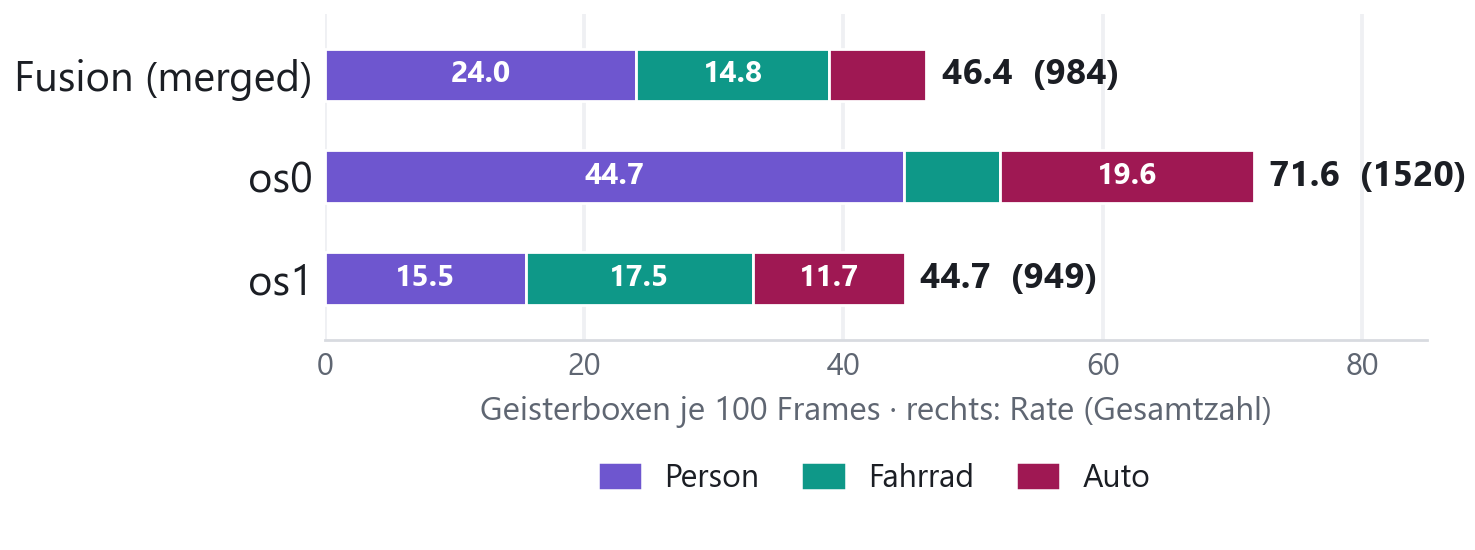
\includegraphics[width=0.95\textwidth]{images/geisterboxen-rate.png}
\caption{Geisterboxen je 100 Testframes, aufgeschlüsselt nach Klasse. Rechts die Gesamtrate mit der absoluten Anzahl in Klammern.}
\label{fig:geisterboxen-rate}
\end{figure}

Die Fehlerbilder unterscheiden sich deutlich zwischen den Ansichten. \texttt{os0} erzeugt mit 71{,}6 Geisterboxen je 100 Frames die mit Abstand höchste Rate, dominiert von Personen- und Autoboxen. \texttt{os1} und \texttt{merged} liegen mit 44{,}7 beziehungsweise 46{,}4 ähnlich, wobei bei \texttt{os1} die Fahrradboxen überwiegen. Die hohe Personen-Geisterboxrate von \texttt{os0} ist die unmittelbare Entsprechung des in Abschnitt~\ref{sec:os0-person} nachgewiesenen Personen-Einbruchs: Beide beschreiben dieselben Fehldetektionen, einmal als absolute Zahl und einmal in ihrer Wirkung auf die Precision-Recall-Kurve.

Dass \texttt{merged} trotz einer geringfügig höheren Rate als \texttt{os1} in allen mAP-Werten vorn liegt, ist kein Widerspruch. Die Geisterboxzählung ist eine absolute Fehlerzahl bei einer festen Konfidenzschwelle von 0{,}3 und keine Precision-Angabe. Die AP integriert dagegen über die gesamte Precision-Recall-Kurve und honoriert zusätzlich gefundene richtige Objekte. Die fusionierte Ansicht erzeugt mehr Vorhersagen insgesamt, darunter sowohl mehr Treffer als auch geringfügig mehr Fehldetektionen. Für den praktischen Betrieb bleibt die absolute Rate dennoch relevant, weil sie die Nachbearbeitung durch Tracking und Betriebsschwellen bestimmt.

\subsection{Plausible Ursachen}
\label{sec:ursachen}

Die detaillierte Fahrradforensik zeigt drei wiederkehrende Gruppen:

\begin{enumerate}
    \item Reale statische oder nicht gelabelte Strukturen werden als Fahrrad interpretiert.
    \item Sparse Reflexions- und Unterbodenpunkte können lokale Aktivierungen auslösen.
    \item Vorhersagen treten wiederholt an Positionen auf, an denen Fahrräder in den Trainingsaufnahmen vorkamen. Dies deutet auf eine ortsgebundene Szenenmemorierung hin.
\end{enumerate}

Ein Filter für Punkte unterhalb des Bodens reduzierte die Geisterboxen in einer Ablation nicht. Daraus folgt lediglich, dass Unterbodenpunkte allein den Effekt nicht erklären; Reflexionen, die oberhalb des Bodens entstehen, werden von dieser Ablation nicht erfasst und bleiben als Teilursache möglich.

Teilweise ragen Fahrrad- oder Personenboxen in die Ground-Truth-Box eines Autos. Das ist als klassenübergreifende Mehrfachhypothese plausibel: Dünn abgetastete Fahrzeugkanten oder das Heck können gleichzeitig einen fahrradähnlichen Anchor aktivieren. Die standardmäßige Non-Maximum Suppression arbeitet klassenweise. Eine korrekte Autobox unterdrückt deshalb keine zusätzliche Fahrradbox. Da die Zusatzbox keine Fahrrad-GT trifft, zählt sie in der Fahrradwertung als False Positive, auch wenn sie ein Auto überlappt.

Eine getestete Cross-Class-NMS entfernte vollständig enthaltene klassenübergreifende Zusatzboxen und veränderte die Metriken nicht. Sie ist als Ausgabebereinigung vertretbar, sollte aber nicht nachträglich anhand der Cross-Validation-Testdaten optimiert werden.

\subsection{Praktische Gegenmaßnahmen}

Für eine spätere Anwendung bieten sich folgende Maßnahmen an:

\begin{itemize}
    \item pro Klasse auf Validierungsdaten gewählte Konfidenzschwellen,
    \item zeitliche Trackbestätigung statt Entscheidungen aus einzelnen Frames,
    \item Hintergrundunterstützung oder eine statische Szenenkarte,
    \item Cross-Class-NMS als konservative Ausgabebereinigung,
    \item zusätzliche Trainingsszenen zur Verringerung der Ortsmemorierung.
\end{itemize}
